\section{Analyse}

\subsection{Problemraum und Anforderungen}
Für den Empfang von Messdaten und die korrekte Startvorbereitung benötigt eine Radiosonde von GRAW auch immer eine Bodenstation.
Auf Bodenstationen läuft unter Windows die Software \enquote{GRAWMET}\cite{grawmet}, welche die Daten der Sonde empfängt, weiterverarbeitet und auswertet.
Um vergangene Flüge auszuwerten und zu überwachen ist daher immer der Zugang zum Bodenstationscomputer notwendig.
Eine zentrale und einfache Auswertung mehrerer Stationen durch Nutzer an verschiedenen Orten mit verschiedenen Endgeräten ist aktuell kaum möglich.
Es gibt für diese Anforderungen bereits eine experimentelle Anwendung \enquote{GRAWgo}\cite{grawgo}, welche aufgrund ihrer Architektur kein On-Premises Hosting unterstützt und nur auf Mobilgeräten lauffähig ist.
GRAWgo hat es, vermutlich aufgrund seiner sehr eingeschränkten Nutzbarkeit, bisher nicht in einen produktiven Betrieb im Bereich von größeren Messnetzen geschafft und ist dafür auch aktuell nicht konzipiert.

Diese Probleme soll durch eine neue Architektur, bzw.\ eine ergänzende Software namens \enquote{Sounding Console}, gelöst werden.
Der Zugang zu den erfassten Daten und Auswertungen soll vereinfacht werden und von verschiedenen Orten aus möglich sein.
An dieser Problemstelle setzt die Sounding Console an und soll die sich daraus ergebenden Anforderungen erfüllen.

Grundsätzlich wurden durch den Auftraggeber Anforderungen im Rahmen eines Lastenheftes (\ref{subsec:lastenheft}) kommuniziert, diese wurden teilweise, nach technischer Einordnung durch den Verfasser dieser Arbeit, angepasst und ergänzt.
Anschließend wurde durch die auftragnehmende Agentur ein Angebot (\ref{subsec:angebot}) erstellt.
Nach Auftragseingang wurden konkretere Anforderungen und daraus resultierende Aufgaben durch den Entwickler, im sogenannten Leistungspaket (\ref{subsec:leistungspaket}), festgelegt.
Teilweise wurden in diesem Prozess offene Fragen mit dem Auftraggeber geklärt.

Im folgenden sind die Anforderungen gelistet, die die neue Software erfüllen soll.
Eine ausführlichere Darstellung findet sich im Anhang dieser Arbeit.
\newpage

\subsubsection{Inhaltliche Anforderungen}
Die inhaltlichen Anforderungen wurden überwiegend seitens des Auftraggebers erarbeitet, ergaben sich aber auch teilweise erst auf konkrete Rückfragen im Entwicklungsprozess.
\begin{itemize}
    \item Administratoren müssen Nutzern den Zugriff ermöglichen können und diesen durch eine Rollenzuweisung mit unterschiedlichen Zugriffsrechten weiter einschränken können.
    \item Im System müssen mehrere Stationen verwaltet werden können, deren Sichtbarkeit muss auf spezifische Nutzer eingeschränkt werden können.
    \item Die Flugdaten müssen via Schnittstelle, von mehreren Bodenstationen gleichzeitig, empfangen werden können.
    \item Die Kommunikation mit Bodenstationen soll nahezu in Echtzeit funktionieren.
    \item Es sollen Flüge und deren Messdaten, aus bestehenden Archiven, importiert werden können.
    \item Eine sprachliche Internationalisierung muss möglich sein.
    \item Je Flug, müssen eindimensionale Performancekriterien berechnet und anzeigt werden können.
    \item Die Performance einer Station soll, mittels durchschnittlicher Performancekriterien aus vergangenen Flügen, in unterschiedlichen Zeitabschnitten, einsehbar sein.
    \item Flugdaten sollen in Echtzeit verfolgt werden können und müssen im Nachhinein ausgewertet werden können.
    \item Es soll eine Kartendarstellung von einem oder mehreren Flügen geben.\ Dafür soll der Einsatz eines Open Source Projektes\cite{sondehub-tracker} geprüft werden.
    \item Für einen Flug müssen Messdaten tabellarisch dargestellt werden können.
    \item Einige Messdaten müssen, je Flug, in zweidimensionalen Liniendiagrammen, gegenüber Zeit/Höhe/Luftdruck, dargestellt werden können.
    \item Es soll geprüft werden, ob mit überschaubarem Aufwand, thermodynamische Diagramme dargestellt werden können.
\end{itemize}
\newpage

\subsubsection{Technische Anforderungen}
Die technische Anforderungen werden von beiden Parteien gemeinsam festgelegt.
Dabei werden die vorhandenen Kompetenzen und Erfahrungswerte, mit Programmiersprachen und Frameworks, seitens des Entwicklers berücksichtigt.
Bei einigen Entscheidungen wird außerdem berücksichtigt, dass die Entwicklung mit möglichst geringen finanziellen Ressourcen erfolgen kann.
\begin{itemize}
    \item Die Software muss auf einer zentralen Instanz gehostet werden, dies muss sowohl auf zentralen Servern als auch On-Premises möglich sein.
    \begin{itemize}
        \item Es sollen aktuelle Standards wie Docker und Kubernetes verwendet werden.
    \end{itemize}
    \item Die Sounding Console soll gegenüber GRAWgo eine bessere Zugänglichkeit und UX aufweisen, insbesondere die Nutzung an einem Desktop Computer soll ermöglicht werden.
    \begin{itemize}
        \item Das System soll webbasiert umgesetzt und deployed werden.
        \item Das Interface soll responsive auf verschiedene Endgerätegrößen reagieren.
    \end{itemize}
    \item Die Software soll durch die Verwendung moderner, bekannter sowie quelloffener Frameworks entwickelt werden.
    \item Durch die Verwendung von Industriestandards soll eine externe Abhängigkeit gegenüber dem Auftragnehmer verhindert werden.
    \item Die sprachliche Internationalisierung soll, durch die Erstellung und Einbindung neuer Sprachdateien effizient möglich sein.
    \item Das Projekt muss mittels git versioniert werden.
    \item Automatische Deployments sollen schnelle Updates der Test- und Produktivumgebung ermöglichen.
\end{itemize}

\subsection{Themenfeldanalyse}
Die folgende visuelle Analyse (\ref{fig:themenfeldanalyse}) gibt einen besseren Überblick über das Themenfeld, welches sich aus der zentralen Projektfrage ableiten lässt.
Außerdem werden übliche sowie grundsätzlich geeignete technische Frameworks betrachtet, die im Projektverlauf von Vorteil sind.

\newpage
\begin{figure}[h!]
    \centering
    \caption{Themenfeldanalyse}
    \label{fig:themenfeldanalyse}
    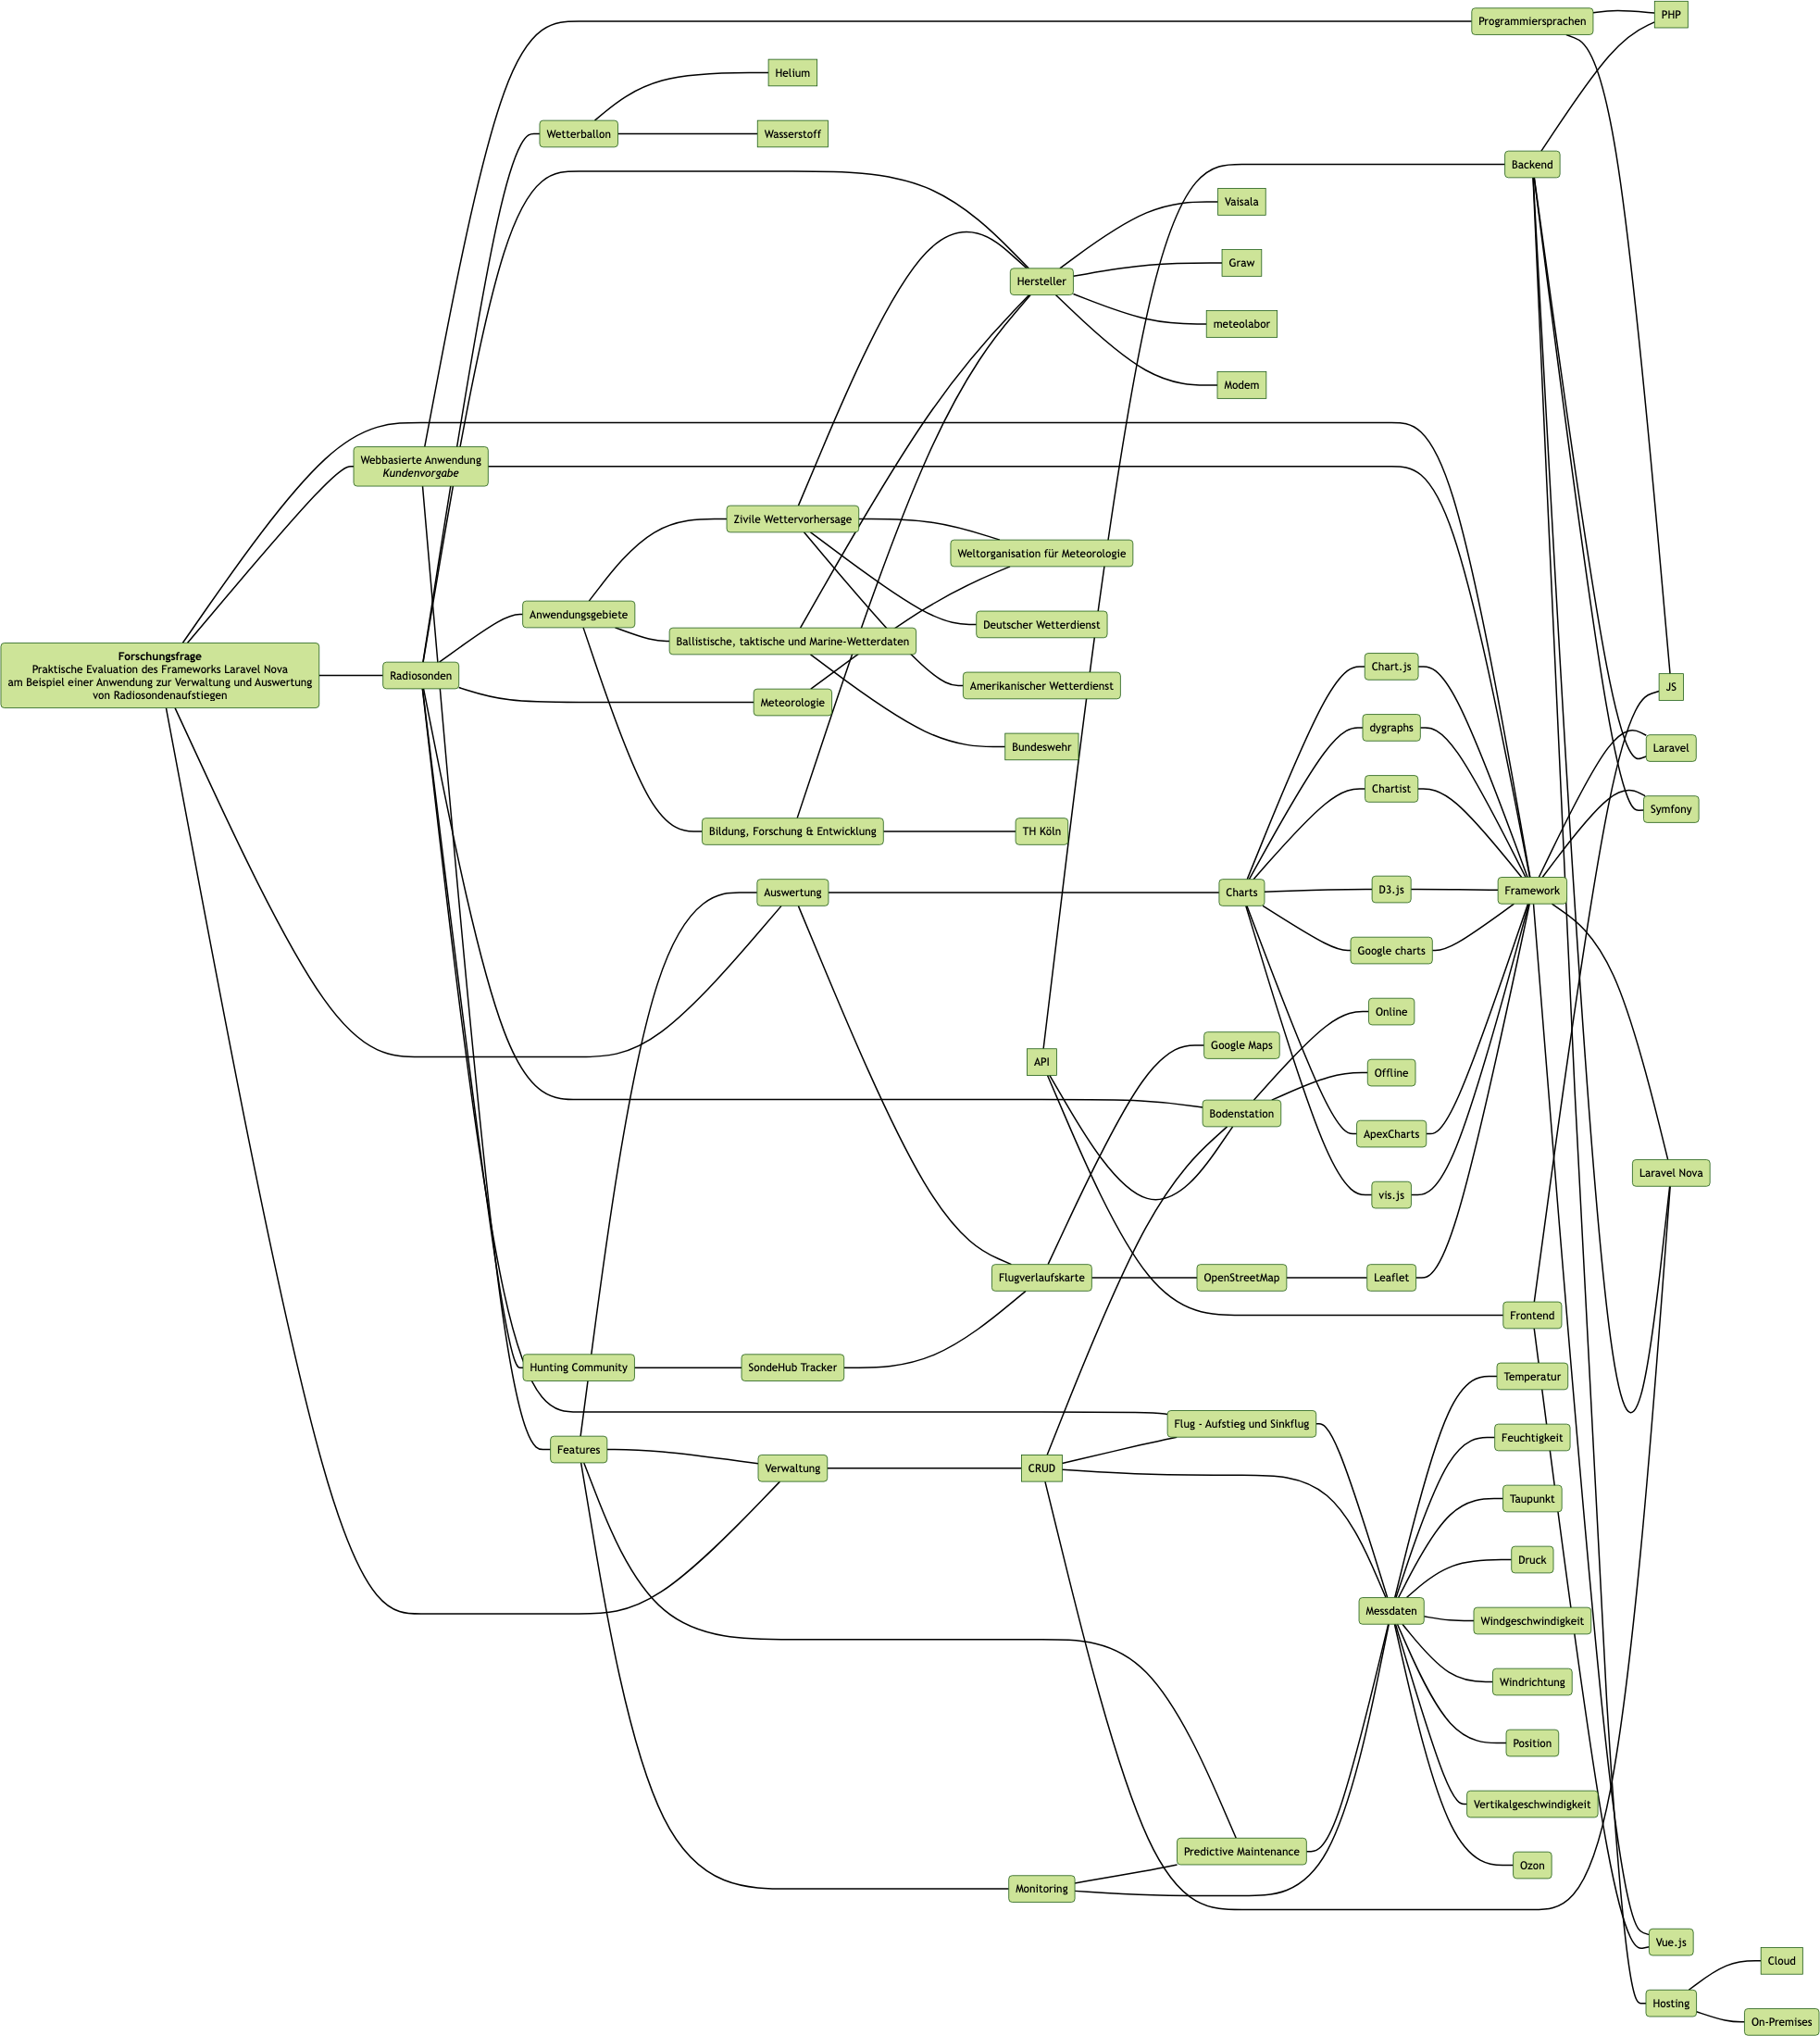
\includegraphics[scale=0.255]{assets/themenfeldanalyse_no_padding}
\end{figure}
\newpage
